% ==================================================
% CHAPTER 2: High energy particle physics %
% ==================================================

\chapter{High energy particle physics}
\label{chap:hep}
% Edit count: Lia - 1, Brigitte - 0

Particle physics aims to study the elementary constituents of matter. Understanding the fundamental building blocks and how they interact provides insight into how the early universe evolved to the forms of matter we observe today. This chapter introduces general concepts in particle physics relevant to understanding the physics goals of the High-Luminosity LHC (HL-LHC) and NSWs upgrade. 

The information on particle physics and the SM presented here is rather general; the interested reader is referred to~\cite{griffiths_introduction_2011, peskin_introduction_1995, zyla_review_2020} for more information. 

% --------------------------------------------------
\section{The Standard Model}
% --------------------------------------------------

The Standard Model (SM) is a theoretical framework developed in the early 1970's that describes the observed elementary particles and their interactions.  It is built on a collection of quantum field theories and has been remarkably successful at predicting experimental observations, including but not limited to the existence of the top quark~\cite{kobayashi_cp-violation_1973}, the tau neutrino~\cite{perl_evidence_1975} and the Higgs boson~\cite{englert_broken_1964, higgs_broken_1964}. 

\begin{figure}
    \centering
    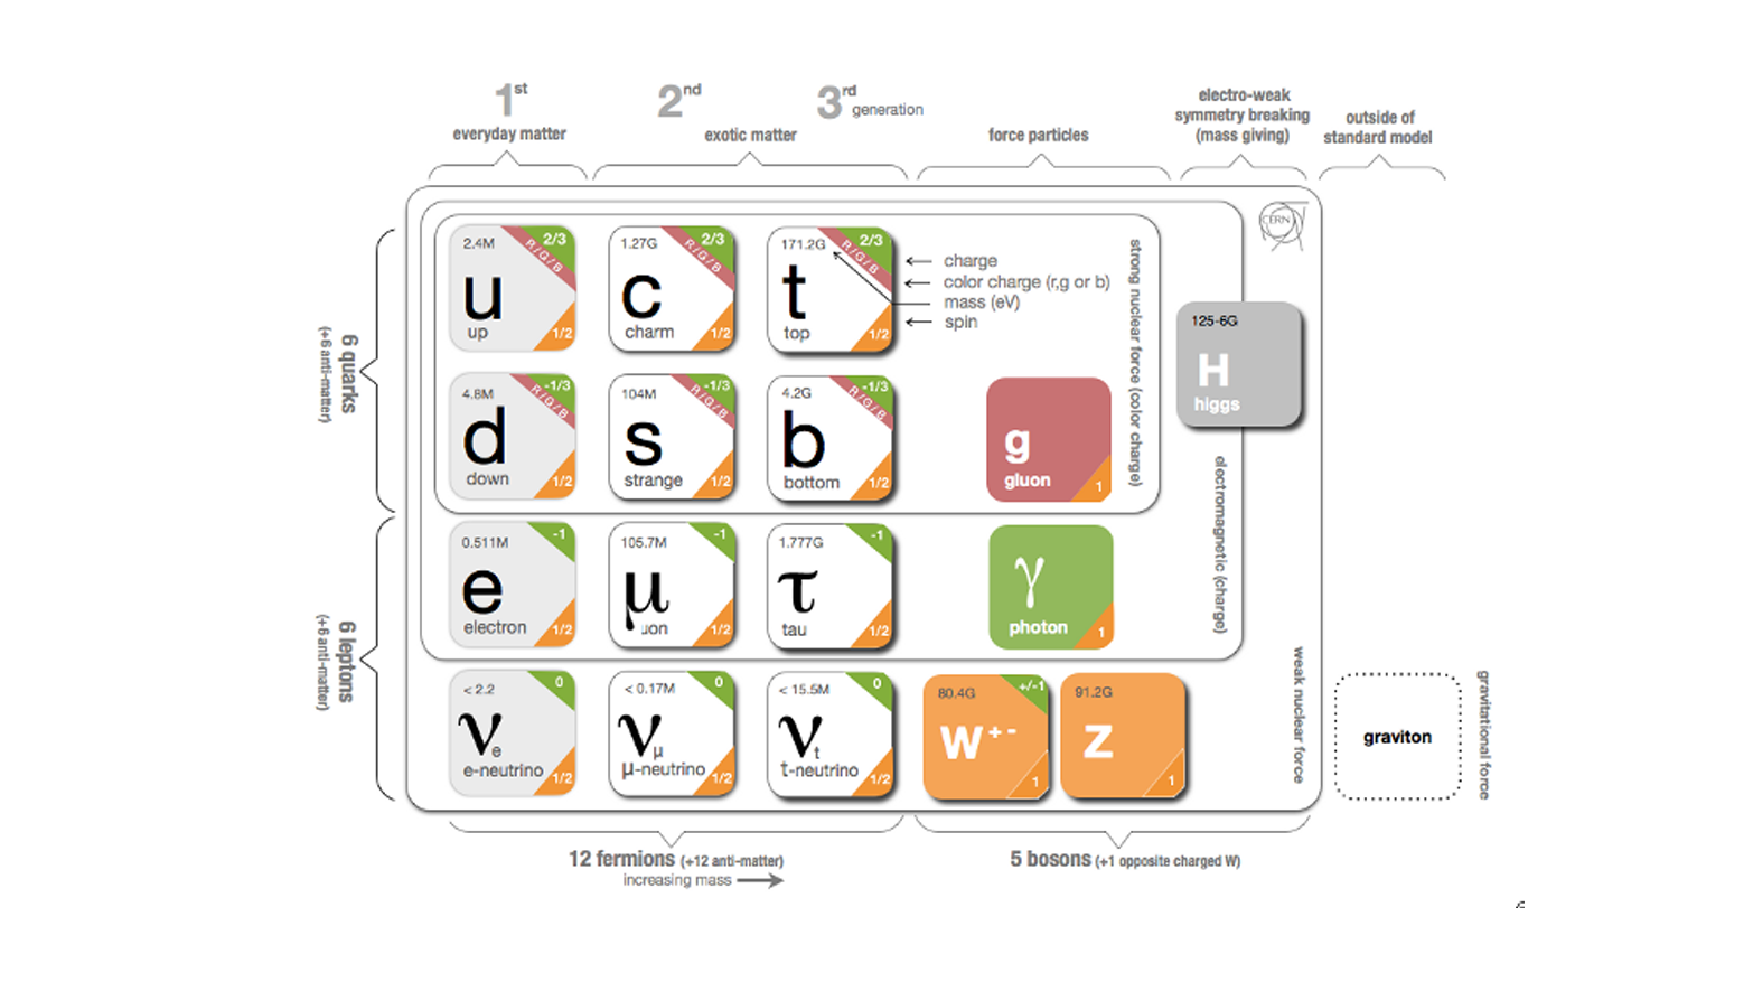
\includegraphics[width = \textwidth]{figures/standardmodel_galbraith_carsten.pdf}
    \caption{Schematic diagram of all elementary particles in the SM.  Particles are grouped according to their properties and the forces through which they interact with other particles~\cite{galbraith_ux_2013}.}
    \label{fig:standard_model}
\end{figure}

The known elementary particles described by the SM are represented in figure~\ref{fig:standard_model}.  There are 12 matter particles (six quarks and six leptons), 4 force-mediating particles, and the Higgs boson. Each matter particle also has an anti-matter particle pair with the same mass but opposite charge, not represented in figure~\ref{fig:standard_model}. The different forces of nature are understood to be the result of the exchange of force-mediating particles between interacting (coupled) particles. Photons are mediators of the electromagnetic force, W+/- and Z bosons are mediators of the weak force, and gluons are mediators of the strong force\iffalse[GRIFFITHS]\fi. At high energy, the SM describes the electromagnetic and weak forces as stemming from a unified electroweak force\iffalse[PESKIN]\fi. The Higgs boson field interacts with the particles mediating the unified electroweak force to distinguish the weak and electromagnetic forces from each other at lower energies and give particles (except neutrinos) a mass. This is called electroweak symmetry breaking\iffalse[PESKIN]\fi. 

Quarks are matter particles that are sensitive to all forces; notably they are the only particles sensitive to the strong force\iffalse[GRIFFITHS]\fi. Protons and neutrons are made up of quarks and gluons, and the strong force is responsible for their existence and mutual attraction into nuclei~\cite{bertulani_nuclear_2007}. Leptons are particles not sensitive to the strong force. Charged leptons include the electron, which once part of atoms is responsible for chemistry. Of particular importance for this thesis is the charged lepton called a muon. It is like the electron but its mass is $\sim$200 times larger than that of the electron. Muons have a lifetime of \SI{2.2}{\micro\second}~\cite{zyla_review_2020} and decay predominantly as $\mu \rightarrow e^{-}\overline{\nu}_{e}\nu_{\mu}$ .Neutrinos are neutral, almost massless leptons that only interact through the weak force\iffalse[GRIFFITHS]\fi. 

Common matter is made up of the lightest constituents of the SM: up and down quarks, electrons and photons. The other particles are produced in high-energy environments but then decay to the lightest constituents. Such high energy environments include the conditions present in the early universe~\cite{carroll_introduction_2007}, astrophysical sources, and particle accelerators\iffalse[REV PART PHYS, GRIFFITHS]\fi. The presence of the particles of the SM at the beginning of the Universe means that their interactions and decays are fundamental for the study of the evolution of the early universe~\cite{carroll_introduction_2007}. Many high energy astrophysical sources, like supernovae, generate particles that rain down on Earth as cosmic rays~\cite{boezio_chemical_2012}\iffalse[BOEZIO, REV PART PHYS, GRIFFITHS]\fi. Particle accelerators have been built to create controlled environments of high-rate, high-energy particle collisions at high energy where the production and decay of elementary particles can be directly studied\iffalse[GRIFFITHS, REV PART PHYS]\fi.

% --------------------------------------------------
\section{Beyond the Standard Model}
% --------------------------------------------------

Despite its success at describing most experimental observations to date, there is ample evidence that the SM is not a complete description of natural phenomena at the smallest scales. For example, the SM has a large number of free parameters, the values of which have to be fine-tuned to fit experimental observations. This is part of the so-called ``naturalness'' problem.

Furthermore, the SM provides no explanation for several open questions in particle physics. First, neutrinos in the SM are assumed to be massless and do not gain mass in the same way as the other particles. However, neutrino were confirmed to change between their different flavours in 2013~\cite{aharmim_combined_2013}, which can only occur if neutrinos do have mass~\cite{pontecorvo_neutrino_1967}. The neutrino mass requires physics beyond the standard model~\cite{bilenky_massive_1987}. Second, several astrophysical and cosmological measurements suggest the presence of ``dark matter'' making up 85~\% of the matter content of the universe~\cite{young_survey_2017}. The nature of dark matter is unknown and so far there is no SM explanation~\cite{munoz_dark_2004}. Third, the SM does not explain the origin and nature of the matter-antimatter asymmetry that produced our matter-dominated universe. Finally, the SM does not include a description of gravity.

Theoretical extensions beyond the Standard Model (BSM) aim to address some of these questions, often predicting existence of yet-unseen elementary particles or physics phenomena beyond those predicted by the SM. These hypothetical new physics phenomena or new particles can be searched for at particle accelerators. 
%For example, super-symmetry (SUSY) predicts that each SM particle has a heavier super-symmetric partner. SUSY would explain the origin of dark matter with weakly interacting massive particles, would solve the so-called ``naturalness'' problem in the SM~\cite{jungman_supersymmetric_1996}. 

% --------------------------------------------------
\section{Studying high energy particle physics with accelerators}
% --------------------------------------------------

In particular, particle accelerators of increasingly higher energy have a long history of enabling the discovery of predicted particles. These include, for example, the discovery of the W~\cite{arnison_W_1983, banner_observation_1983} and Z bosons~\cite{arnison_Z_1983, bagnaia_evidence_1983}, the top quark~\cite{cdf_collaboration_observation_1995, d0_collaboration_observation_1995}, and most recently, the Higgs boson~\cite{the_atlas_collaboration_observation_2012, the_cms_collaboration_observation_2012}. The discovery of the Higgs boson marked the completion of the SM as it is known today.

Based on the established success of the SM, there are two approaches to particle physics research. One approach is to search for the existence of new physics phenomena predicted to exist in BSM theories and the other is to test the validity of the SM to a high degree of accuracy to search for flaws in the model. Standard Model predictions are generally expressed in terms of the probability of a specific physics process to occur, expressed as a cross section in units of barns (with 1 barn $=$ 10$^{-28}$ m$^{2}$).  As an example, figure~\ref{fig:standard_model} shows a summary of cross section measured for different physics processes using the ATLAS experiment and their comparison with the predictions of the SM. Most cross section measurements agree well within one standard deviation with the SM predictions. 

\begin{figure}
    \centering
    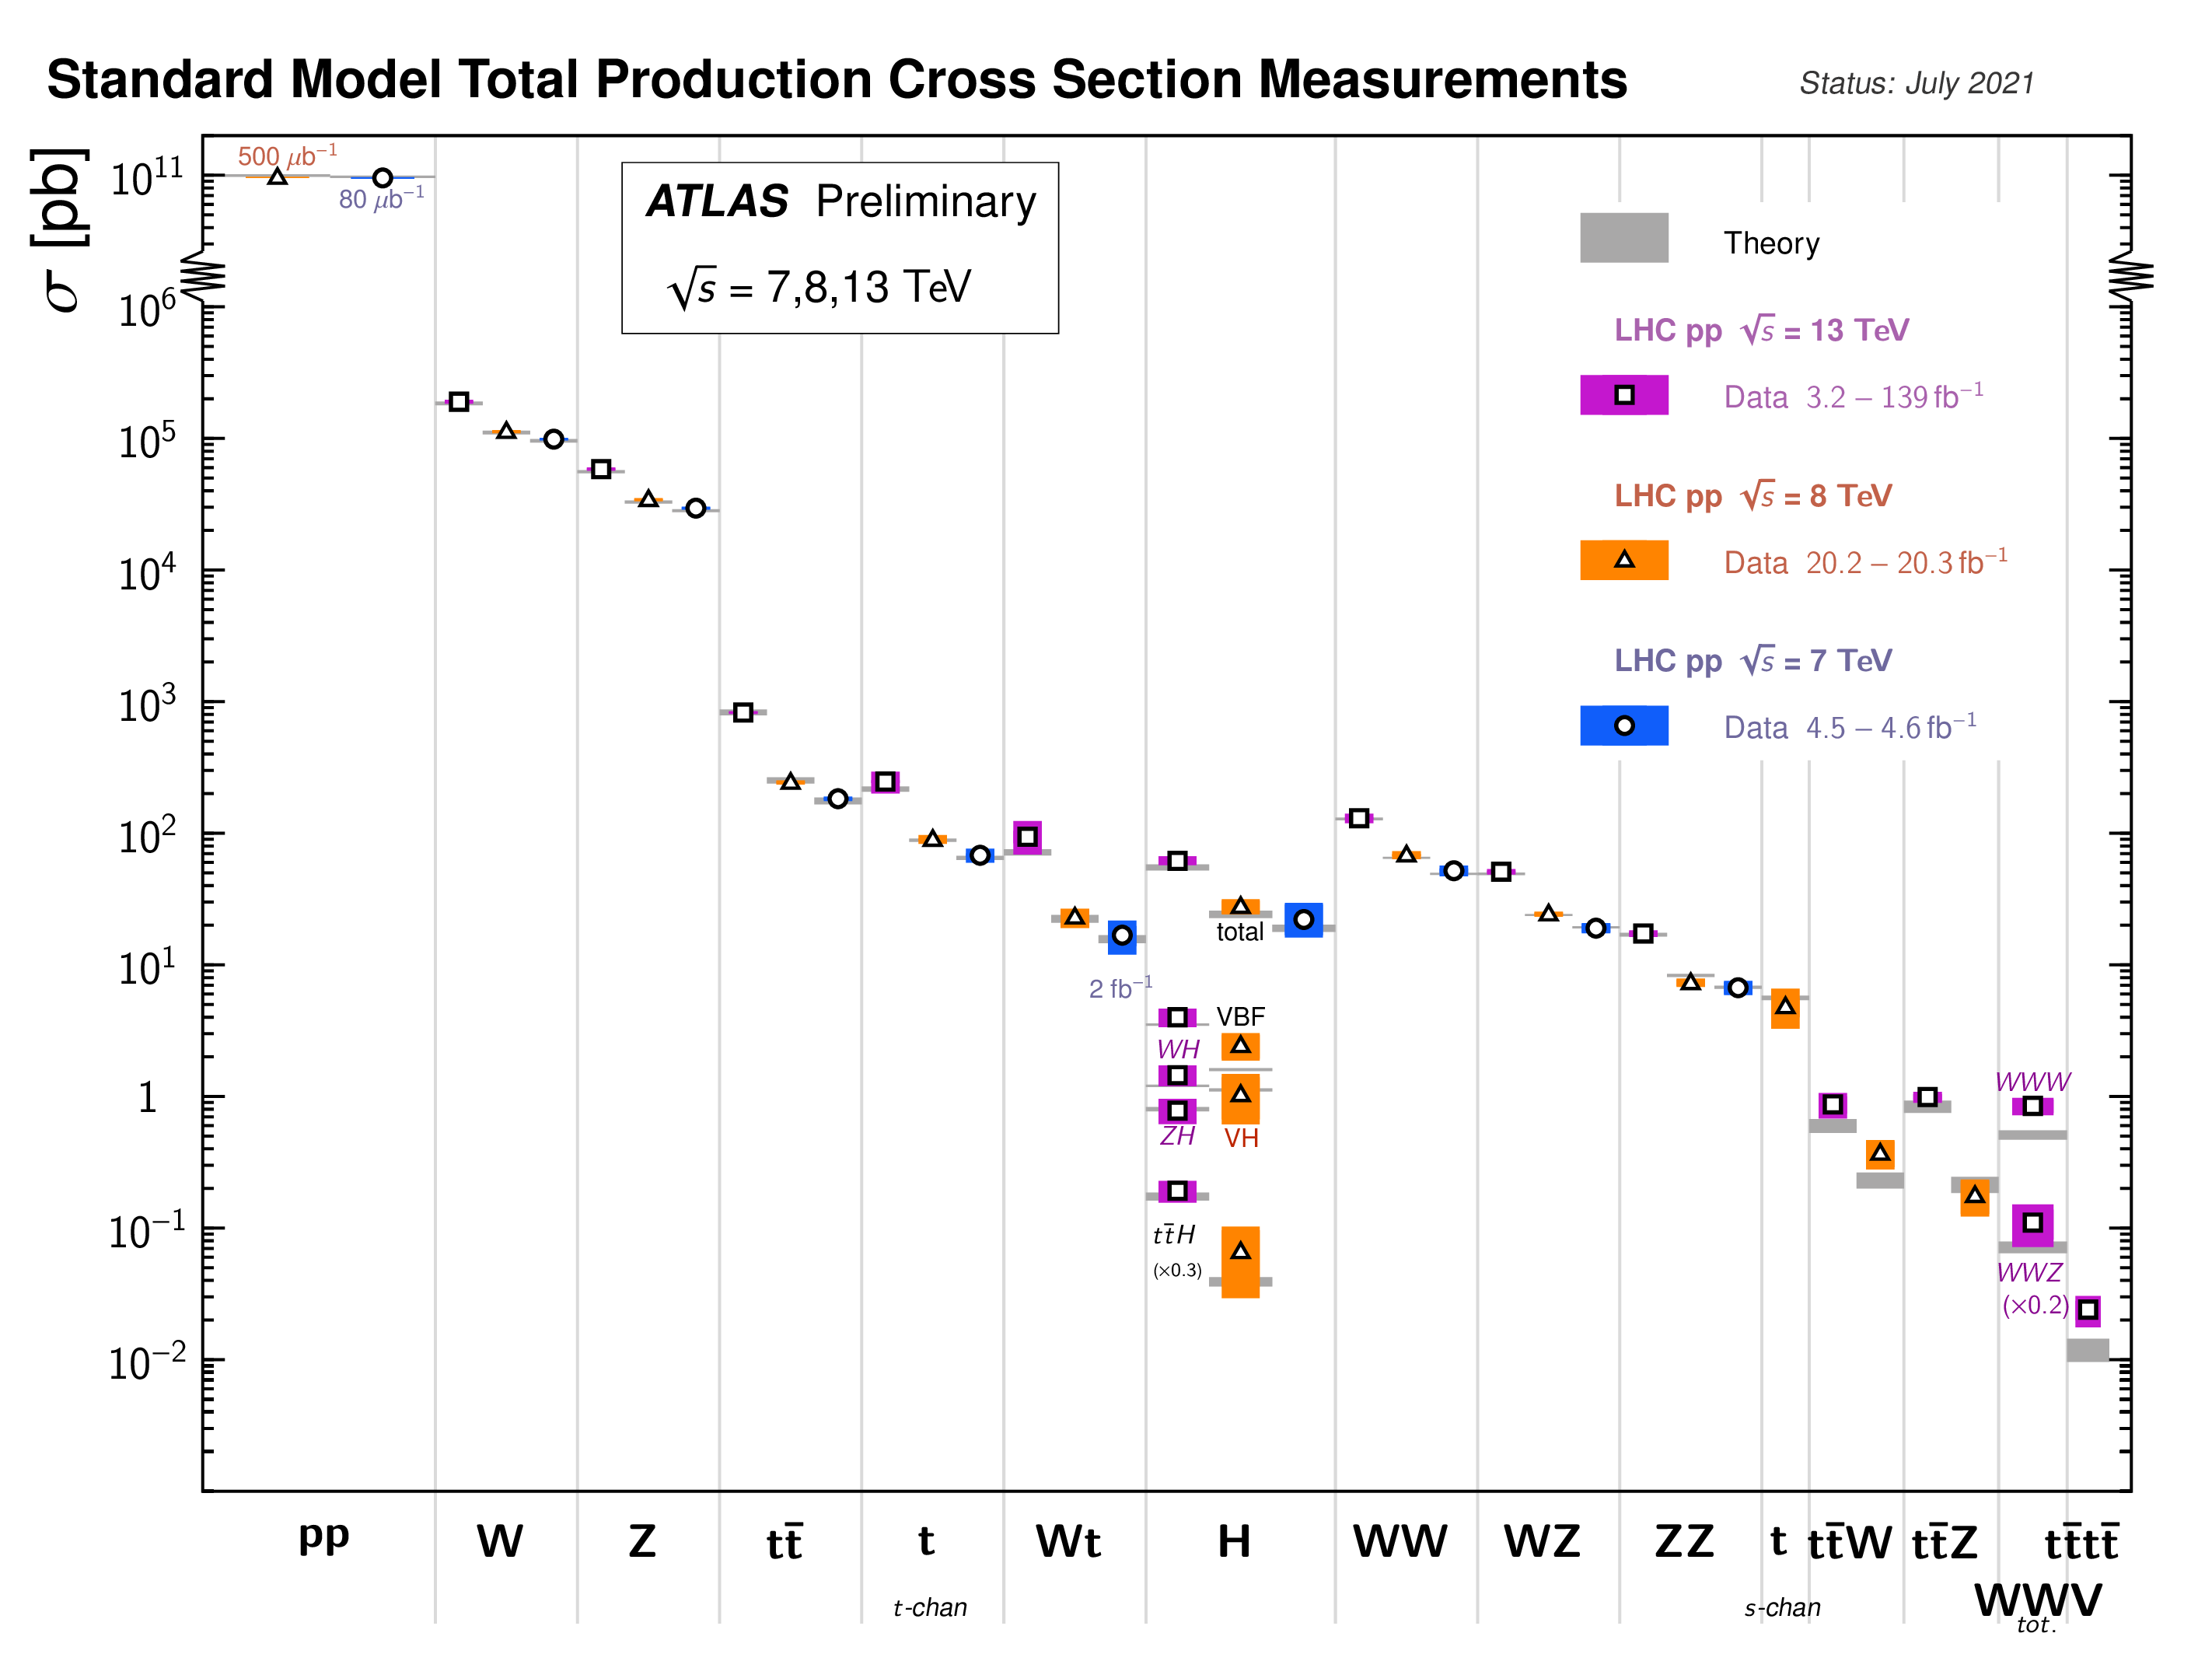
\includegraphics[width = \textwidth]{figures/atlas_cross_sections.png}
    \caption{Production cross sections of different final states measured by the ATLAS experiment at the LHC. Comparison with the SM theory predictions is also shown~\cite{atlas_public_web_sm}.}
    \label{fig:atlas_cross_sections}
\end{figure}

Particle accelerators provide a controlled and high-collision rate environment that makes them ideal places to search for new physics phenomena and to carry out systematic tests of the SM. The LHC is the highest energy collider in the world so it can access physics that no other accelerator can. A description of the LHC and the ATLAS detector are provided in the next chapter. 